\documentclass[10pt,twocolumn,letterpaper]{article}
\usepackage{tikz}  % For plots, must be the first include

\usepackage{cvpr}
\usepackage{times}
\usepackage{epsfig}
\usepackage{graphicx}
\usepackage{amsmath}
\usepackage{amssymb}

% Include other packages here, before hyperref.
\usepackage{pgfplots} % For plots
\usepackage{pgfplotstable} % For plots
\pgfplotsset{compat=newest} % For plots
\usetikzlibrary{plotmarks} % For plots

% If you comment hyperref and then uncomment it, you should delete
% egpaper.aux before re-running latex.  (Or just hit 'q' on the first latex
% run, let it finish, and you should be clear).
\usepackage[pagebackref=true,breaklinks=true,letterpaper=true,colorlinks,bookmarks=false]{hyperref}

% \cvprfinalcopy % *** Uncomment this line for the final submission

\def\cvprPaperID{752} % *** Enter the CVPR Paper ID here
\def\httilde{\mbox{\tt\raisebox{-.5ex}{\symbol{126}}}}

\usepackage{algorithmic}	% Nice algorithm environment
\usepackage{algorithm}
\newcommand{\todo}[1]{\textbf{\textcolor{red}{[#1]}}}
\newcommand{\dx}[1]{\textbf{\textcolor{green}{[Dengxin:#1]}}}
\newcommand{\yh}[1]{\textbf{\textcolor{blue}{[Yuhua:#1]}}}
\newcommand{\jd}[1]{\textbf{\textcolor{magenta}{[Jordi:#1]}}}
% \newcommand{\etal}{\textit{et al.}}
\usepackage{bbm}

% Pages are numbered in submission mode, and unnumbered in camera-ready
\ifcvprfinal\pagestyle{empty}\fi
\begin{document}

%%%%%%%%% TITLE
\title{Scale-Aware Alignment of Hierarchical Image Segmentation}

\author{First Author\\
Institution1\\
Institution1 address\\
{\tt\small firstauthor@i1.org}
% For a paper whose authors are all at the same institution,
% omit the following lines up until the closing ``}''.
% Additional authors and addresses can be added with ``\and'',
% just like the second author.
% To save space, use either the email address or home page, not both
\and
Second Author\\
Institution2\\
First line of institution2 address\\
{\tt\small secondauthor@i2.org}
}

\maketitle
%\thispagestyle{empty}

%%%%%%%%% ABSTRACT
\begin{abstract}

Computer vision has leaped forward during the last decade, and now is able to recognize objects of thousands of categories and reconstruct 3D scenes at city- or world-scale. However, the field still has to find means to keep up with the exploration of the massive amounts of data being captured on a daily basis. This is mainly due to the lack of sufficient training annotations and the lack of computational resources. The thesis is dedicated to mitigate the problem.

Firstly, we elaborate two strategies to reduce the annotation costs in order to train vision algorithms: (1) developing smart annotation approaches for efficient, large-scale annotations; and (2) learning better feature representations using unlabeled data;  We develop algorithms for the strategies and show - in the context of recognition tasks - that they are able to considerably reduce the annotation costs for the training of recognition algorithms.

Secondly, in addition to reducing annotation cost, we also examine how to reduce the computational cost associated with the training and testing of recognition algorithms. This research has lead to two contributions: (1) two efficient solvers for linear and kernel SVM+, significant speeding up the training process of SVM+ to explore privileged information; and (2) a method to allow computationally cheap features to imitate alternative features that perform better but are computationally more expensive. The imitation significantly improves the performance of the cheap features while retaining their efficiency.

Thirdly, as images keep growing in size, vision algorithms need to be more intelligent and self-aware of their performance. To this aim, we have developed approaches to predict the performance vision algorithms at two levels of granularity: (1)  \emph{Succeed or Fail?}  and (2) \emph{Under-, Properly-, or Over-Performed?}. The two methods are evaluated on texture synthesis and image segmentation respectively, and their potentials in reducing computational time are examined as well.

\end{abstract}


%%%%%%%%% BODY TEXT
\section{Introduction}

Whereas numerous works have been developed on example-based texture
synthesis (ETS)~\cite{Heeger:95, Portilla:2000:IJCV,
  Efros:sig2001,Kwatra:2003, Lefebvre:2005:sig, Ma:2011,
  dai:facade:iccv13} and are able to generate a variety of textures
from small examples, no one has systematically studied the
synthesizability of a texture example -- how well its underlying
visual patterns can be re-synthesized by learning only from this
example. This is contrary to other image properties that have been
studied, such as image quality~\cite{image:quality},
memorability~\cite{image:memorability},
interestingness~\cite{image:interestingness}. In this paper, we are
interested in learning image synthesizability and verifing its
usefulness in multiple applications.

Texture mapping adds detailed appearance of surface by projecting a
digitized texture image onto a surface. Although the technique itself
is straightforward, acquiring the texture images of desired size and
shape is not trival. The problem is pronounced as current large-scale
graphics applications require massive amounts of such textures. While
ETS has been proven a powerful tool to generate them~\cite{WLKT09},
providing massive amounts of `synthesizable' examples is not a trival
task. ETS systems expect a square image representing a flat,
outlier-free texture surface. 
% , and assume that the single example
% carries sufficient information about the underlying texture patterns
% for re-synthesis. 
The requirement is hard to enforce for large-scale applications:
texture examples obtained from image searching engine (by keywords)
possibly contain outliers, cluttered backgrounds, distorted texture
surfaces, or even objects of other categories. Thus, there is a clear
need to predict the synthesizability of these images in order to
filter out the unsynthesizable ones. Image synthesizability can also
be used to guide an image trimmimg process to make retrieved texture
examples more synthesizable. Also, there is no database with
annotations of the synthesizability of each image.
Fig.~\ref{fig:synlity} shows the synthesizability of some image
examples detected by our system and Fig.~\ref{fig:roi} shows the most
synthesizable regions detected by our system.

 
\begin{figure} [!t]
  \centering
   $ \begin{array}{cccc}
\hspace{-1.5mm}
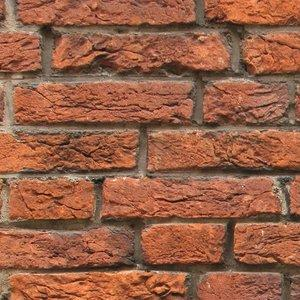
\includegraphics[width=0.33\linewidth]{./figs/1/1.jpg} & 
\hspace{-3mm}
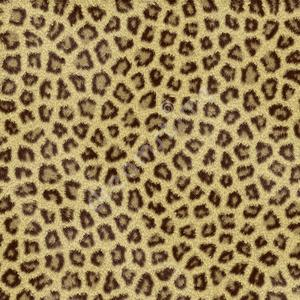
\includegraphics[width=0.33\linewidth]{./figs/1/43.jpg}&
\hspace{-3mm}
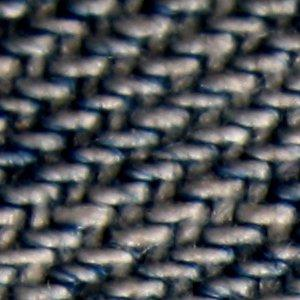
\includegraphics[width=0.33\linewidth]{./figs/1/60.jpg} \\
\scriptsize{\text{\textcolor{red}{0.98}}} & \scriptsize{\text{\textcolor{red}{0.90}}} & \scriptsize{\text{\textcolor{red}{0.85}}} \\
% \hspace{-3mm}
% 455 0.56 feature.jpg 0.66   512 0.41   96 0.44 cliff3.jpg 0.40 
\hspace{-1.5mm}
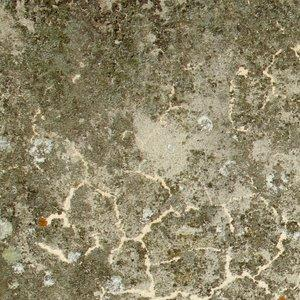
\includegraphics[width=0.33\linewidth]{./figs/1/55.jpg} & 
\hspace{-3mm}
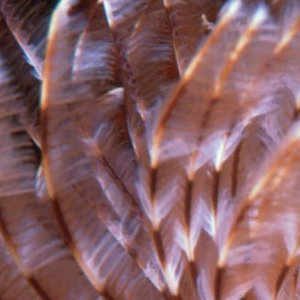
\includegraphics[width=0.33\linewidth]{./figs/1/feather.jpg}&
\hspace{-3mm}
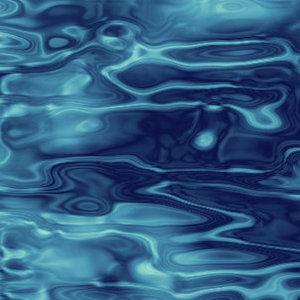
\includegraphics[width=0.33\linewidth]{./figs/1/40ee.jpg} \\
\scriptsize{\text{\textcolor{red}{0.79}}} & \scriptsize{\text{\textcolor{red}{0.66}}} & \scriptsize{\text{\textcolor{red}{0.56}}} \\
\hspace{-1.5mm}
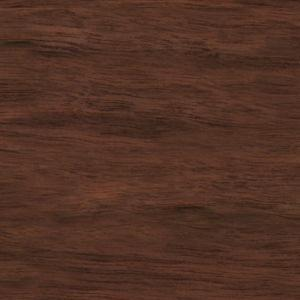
\includegraphics[width=0.33\linewidth]{./figs/1/96.jpg} & 
\hspace{-3mm}
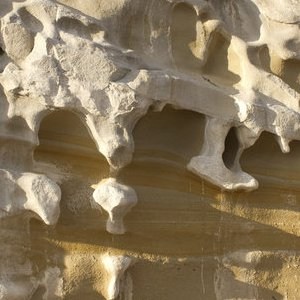
\includegraphics[width=0.33\linewidth]{./figs/1/cliff3.jpg}&
\hspace{-3mm}

\includegraphics[width=0.33\linewidth]{./figs/1/512.jpg} \\
\scriptsize{\text{\textcolor{blue}{0.44}}} & \scriptsize{\text{\textcolor{blue}{0.42}}} & \scriptsize{\text{\textcolor{blue}{0.36}}} \\
\hspace{-1.5mm}

\includegraphics[width=0.33\linewidth]{./figs/1/427.jpg} & 
\hspace{-3mm}
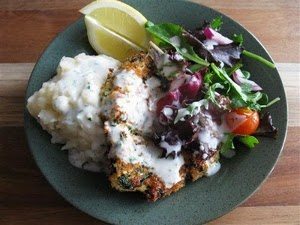
\includegraphics[width=0.33\linewidth, height=27.5mm]{./figs/1/faith4.jpg}&
\hspace{-3mm}
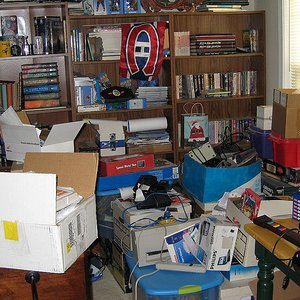
\includegraphics[width=0.33\linewidth]{./figs/1/shelf.jpg} \\
\scriptsize{\text{\textcolor{blue}{0.28}}} & \scriptsize{\text{\textcolor{blue}{0.25}}} & \scriptsize{\text{\textcolor{blue}{0.13}}} \\
% \hspace{-3mm}
% 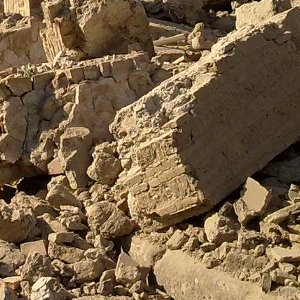
\includegraphics[width=0.25\linewidth]{./figs/1/wall.jpg} \\
\end{array}$
\caption{Synthesizability (Synlity) of texture examples detected by
  our system. All images are of $300\times 300$ pixels.}
  \label{fig:synlity}
\end{figure}


\begin{figure} [!t]
  \centering
   $ \begin{array}{cccc}
\hspace{-1.5mm}
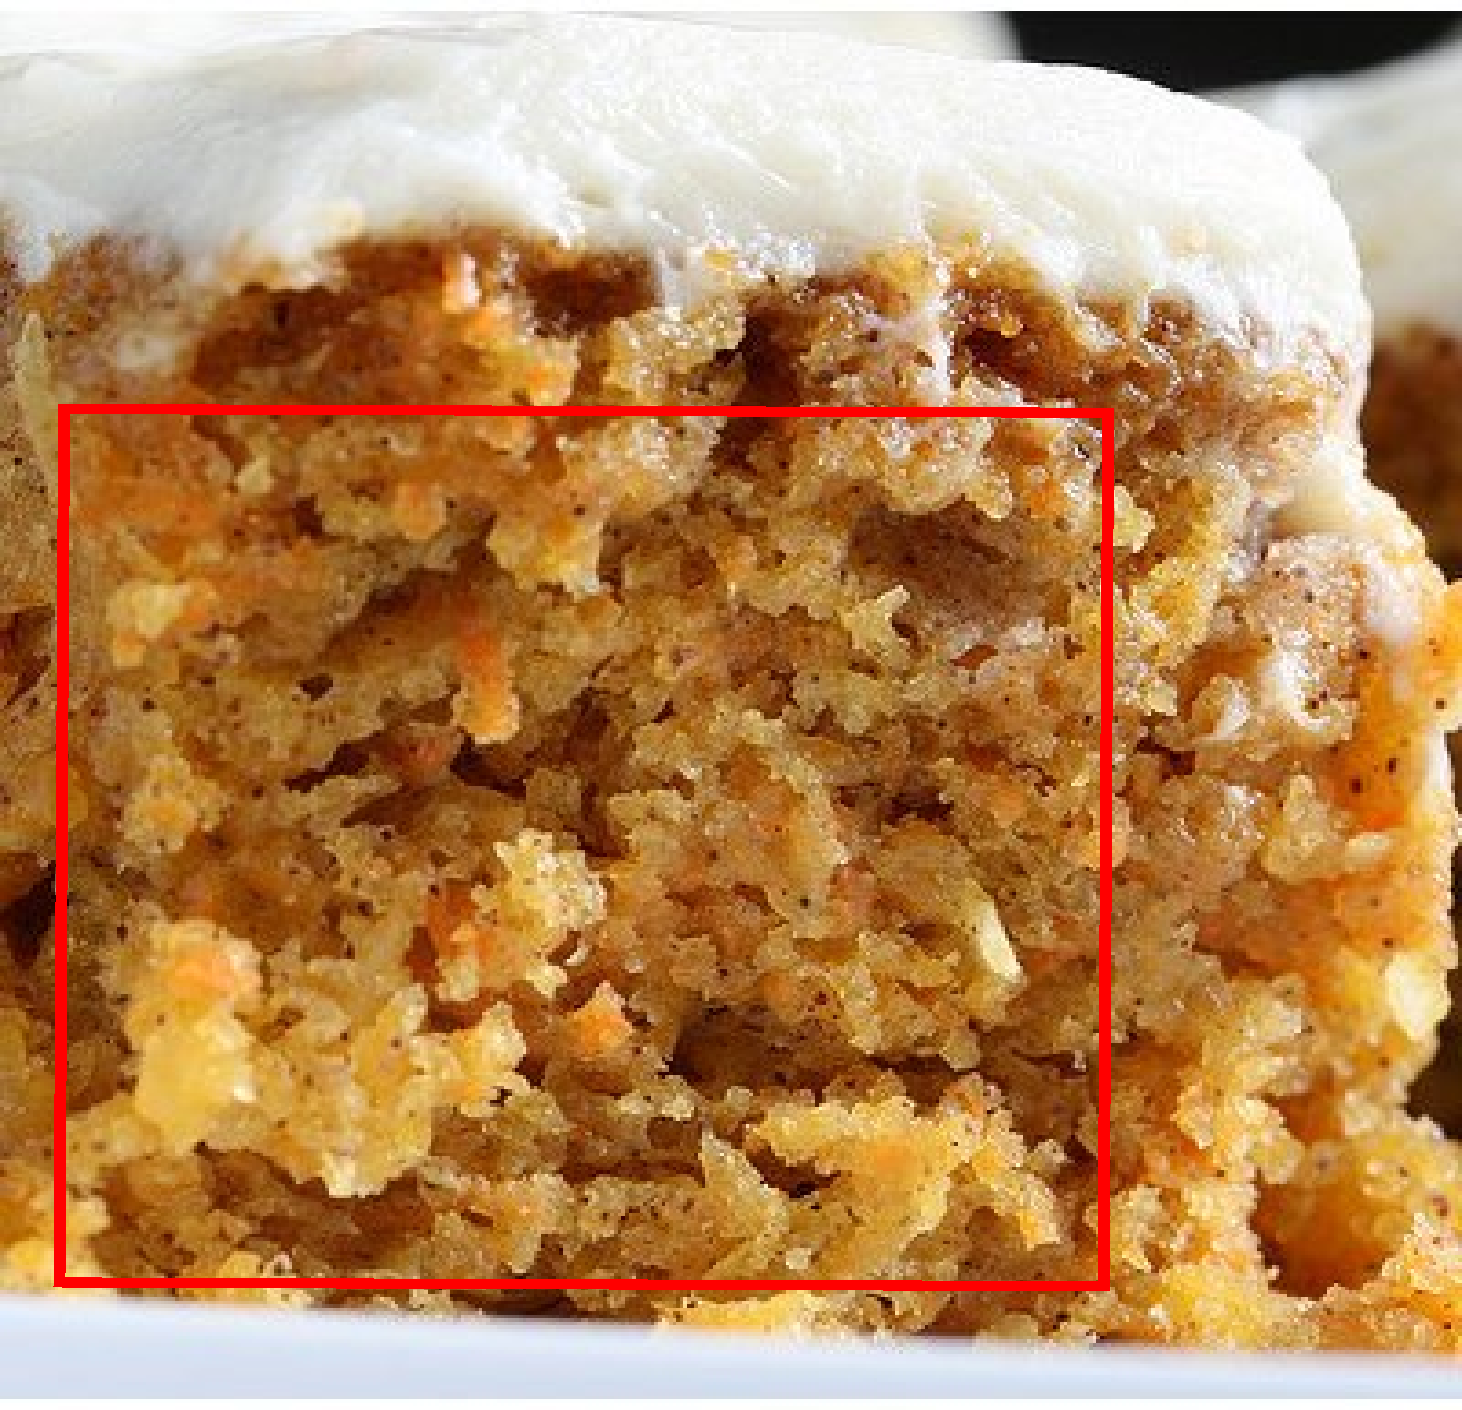
\includegraphics[width=0.48\linewidth, height=35mm]{./figs/2/2.pdf} & 
\hspace{-3mm}
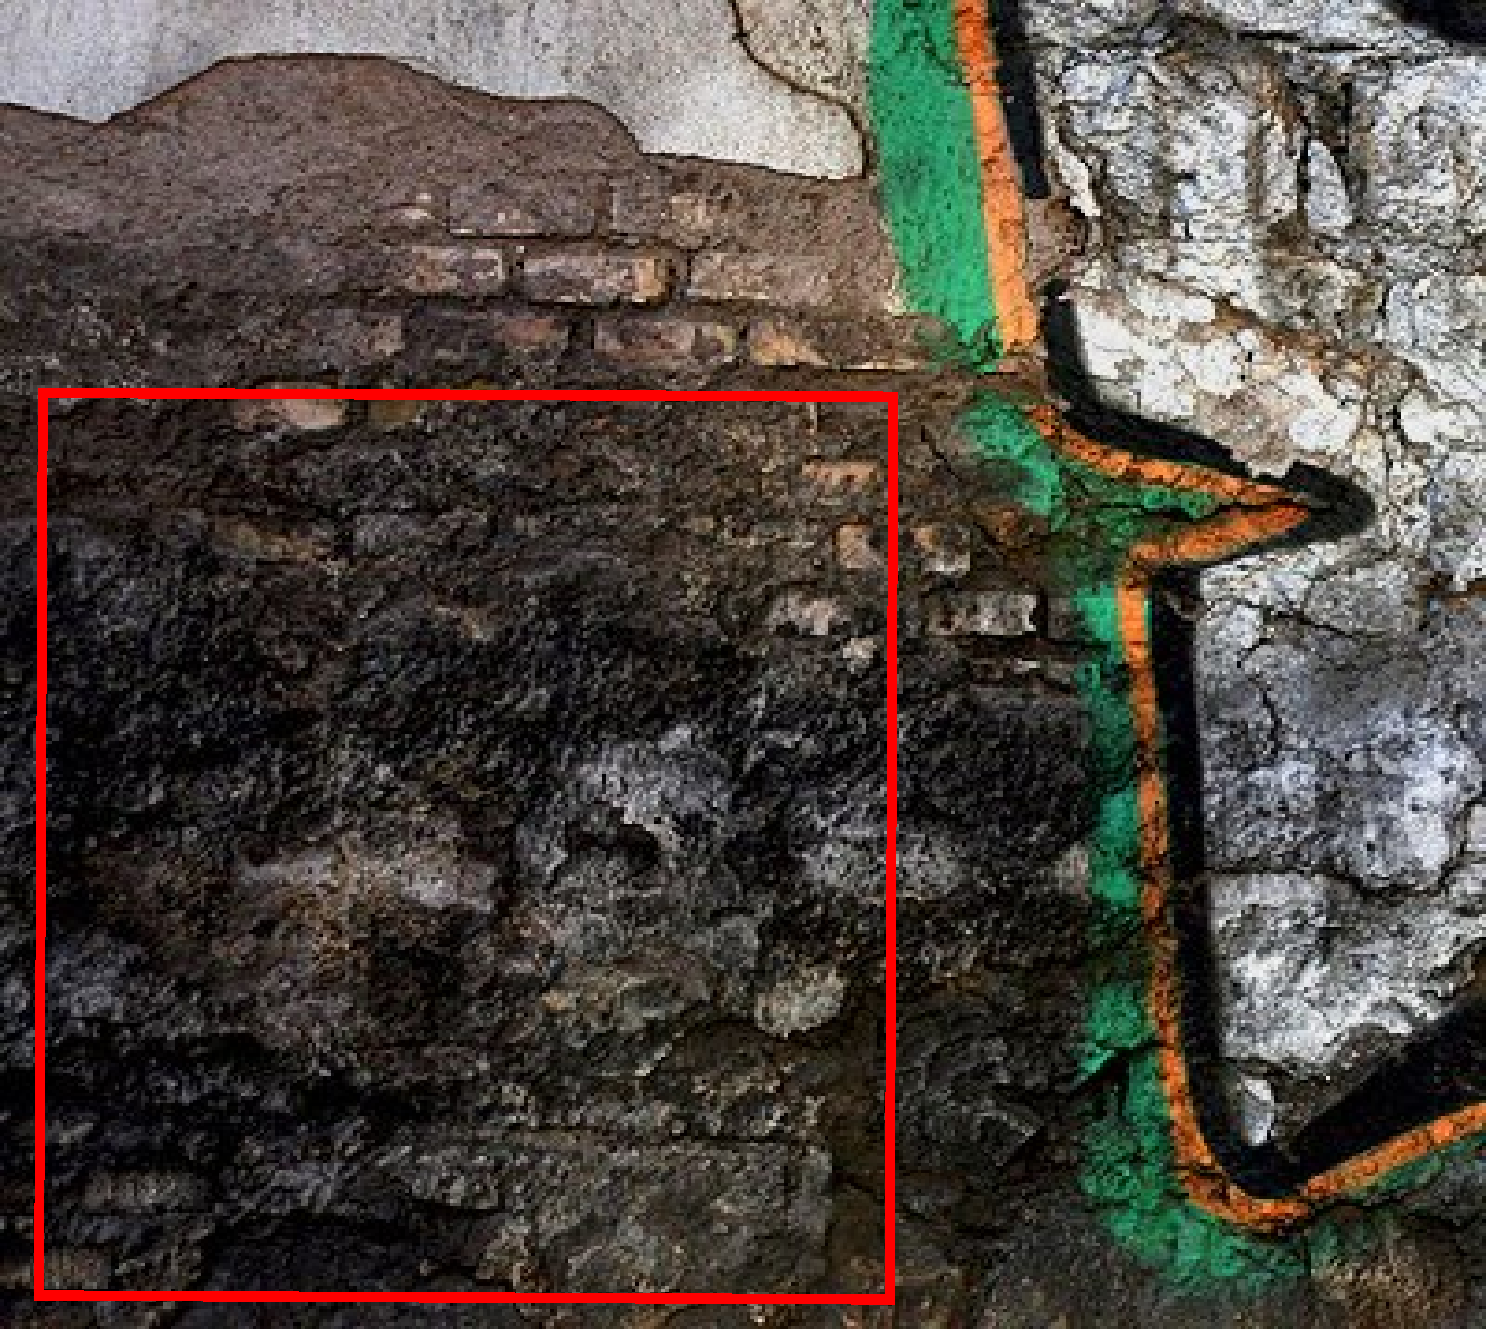
\includegraphics[width=0.48\linewidth, height=35mm]{./figs/2/3.pdf} \\
\scriptsize{\text{r-synlity:\textcolor{red}{0.92} \hspace{1mm} i-synlity:0.40}} & 
\scriptsize{\text{r-synlity:\textcolor{red}{0.67}, \hspace{1mm} i-synlity:0.50}}  \\
\end{array}$
\caption{The most synthesizable region detected by our system. 
Synthesizability of detected regions (r-synlity) and the whole images (i-synlity) are shown. }
  \label{fig:roi}
\end{figure}

In order to learn image synthesizability and evaluate its performance,
a fairly large texture database containing $32,000$ texture images is
constructed, and annotated according to the synthesizability of each
image.  We characterize image synthesizability as the `goodness' of
synthesized textures. A series of features are employed and designed
to computationally capture image synthesizability. Multiple learning
methods are used to learn it from the collection of data. Experimental
result show that image synthesizability is predictable by learning
from a large collection of data. We also show in experiments that
image synthesizability is a general image property and is helpful for
image recognition as well.

Our main contribution are: (1) learn the image property
synthesizability methodologically; (2) design several features for
texture analysis (esp. Repetitiveness, Irregularity); (3) collect a
fairly large texture dataset and annotate it in terms of
synthesizability; (4) verify the usefullness of synthesizability in
multiple vision applications.




\section{Related work}
\textbf{Example-based texture synthesis.} Techniques of example-based
texture synthesis can be broadly categorized into four categories:
feature-oriented image reconstruction~\cite{Heeger:95,
  Portilla:2000:IJCV, random:phase}, Markov Random Fields (MRFs)
methods~\cite{noncausal:tip98, Zalesny05}, tile-based
methods~\cite{Cohen:2003:wang, Liu:2004:NTA}, and
neighborhood-based methods~\cite{Efros:sig2001, Kwatra:tog:2005,
  Kwatra:2003}. The first group learn statistics of a brand of
carefully designed features and coerce the synthetic images to have
the same, e.g. color histograms~\cite{Heeger:95}, wavelet
features~\cite{Portilla:2000:IJCV}, and frequency
spectrum~\cite{random:phase}.  The main difficulty lies in designing a
common set of features that is able to capture the essence of all
kinds of textures.  The second group believe that textures are
instances of MRFs. Parameters of some forms of MRFs are estimated from
the texture examples and new textures are then sampled from the
model. Multi-scale neighborhood-based MRFs are learned
in~\cite{noncausal:tip98} and pairwise clique-based MRFs
in~\cite{Zalesny05}. The third group generate textures by copying
pixels or patches from the exemplar inputs~\cite{Efros:1999,
  Efros:sig2001, Kwatra:2003, Kwatra:tog:2005}. While unlike the first
two groups to provide a key for texture analysis, this group are often
more efficient and tend to work for a larger variety of textures. The
last group assemble new textures out of a set of (rectangular) tiles
croped from example images. It is efficient, but alignment of tiles to
texture elements is often difficult~\cite{Cohen:2003:wang,
  Liu:2004:NTA, dai:facade:iccv13}.

\textbf{Texture recognition.}  Our work is related also related to
texture and material recognition. Efforts have been made mainly on
designing effective features to distinguish textures from different
material categories, including statistics of filter
response~\cite{texton:2001}, the joint intensity distributions within
a compact neighborhood ~\cite{material:pami:09, sorted:texture}, and
the combination of multiple texture features~\cite{material:ijcv13}.
Our system is solving a different task: learning the synthesizability
of texture images instead of their classes. Thus, we need to design
new features for this new task. 

%\section{Critical Levels}

There are around 500 different layers, and XXX regions in a single segmentation tree. Besides, regions in nearby layer can be highly similar. Assessing all of them is both unnecessary and computationally impractical. Therefore, as a pre-processing step, we aim to predict a set of critical levels. These critical levels should be complementary to achieve a high recall to ground truth regions, yet keep the size of set smaller. Similar idea was used in~\cite{krahenbuhl2014geodesic}, where they use critical levels to predict size of segmentation masks.

In order to identify these critical levels efficiently, we train a model based on segmentation entropy features. Segmentation entropy of a segmentation $S$ is defined as:
\begin{equation}
Entropy(S) = \sum_{\textbf{r}\in S}{|\textbf{r}|log(|\textbf{r}|)}
\end{equation}

$|\textbf{r}|$ represents the area of a region $\textbf{r}$ in segmentation $S$. Since only the area is required, segmentation entropy is very fast to compute. It enables us to assess difference between layers of a segmentation tree efficiently, as illustrated in Fig~\ref{fig:entropy}. The steep point on the curve indicates there is a large change in the segmentation.

\begin{figure}
\begin{center}
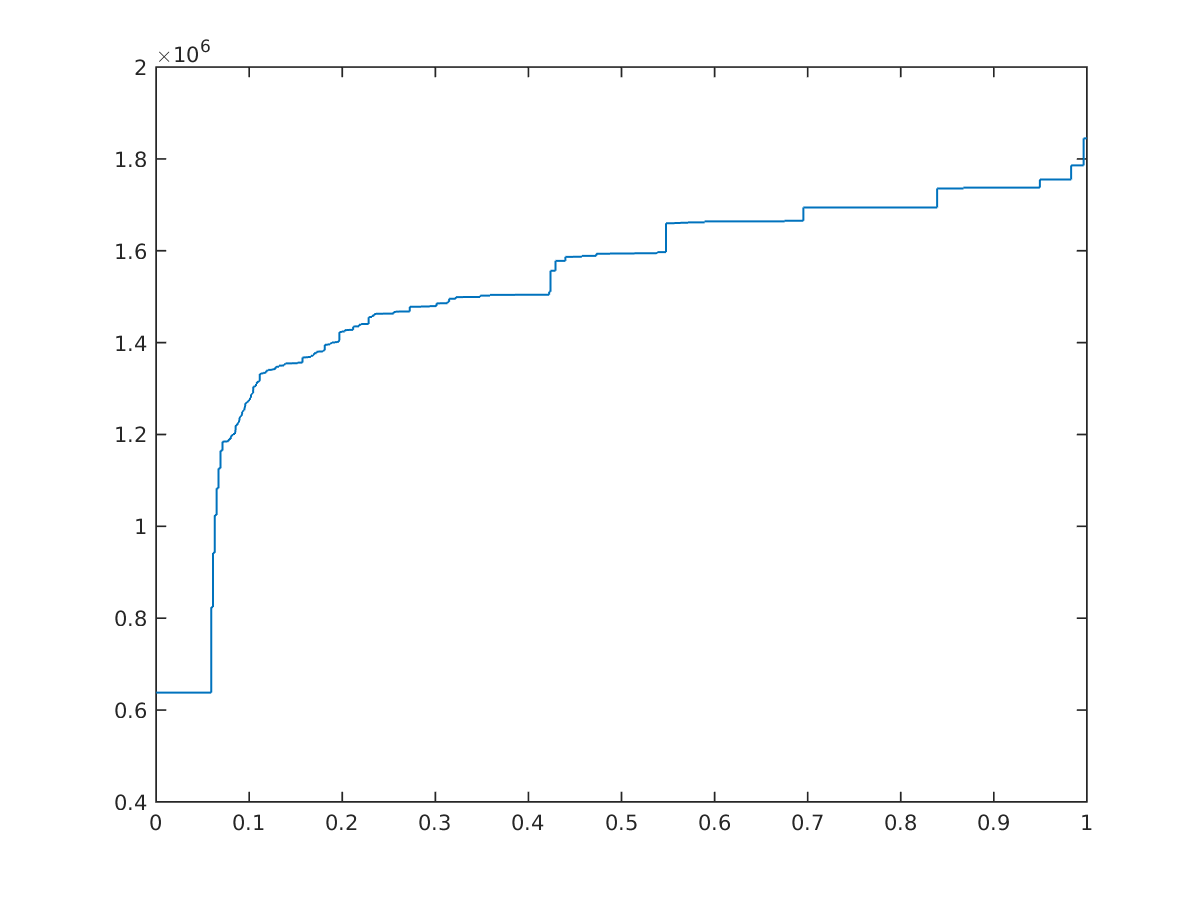
\includegraphics[width=0.5\linewidth]{fig/6046_ucm.png}
\end{center}
\caption{entropy}
\label{fig:entropy}
\end{figure}

The features used includes: value of threshold and entropy, and local gradient of both threshold and entropy calculated with different footstep length. More details about the feature are in the supplementary materials.

\yh{Experiments are not done, will add later}
  
\input{flat_hier.tex}
\section{Experiments}
\label{sec:experiments}
We evaluate our approach on the segmentation hierarchies generated by
multiple different segmentation methods, and further examine its
usefulness on the task of object segmentation. The goal is to
demonstrate that the proposed method is able to improve general
segmentation hierarchies and the improvement is reflected to
high-level vision tasks as well.

% In this section, we present our experiments. First we describe the
% settings of our experiments. Next we incorporate our hierarchy
% alignment with MCG~\cite{arbelaez2014multiscale}, which is
% state-of-the-art hierarchical segmentation method. We report our
% results on the BSDS500 dataset~\cite{arbelaez2011contour}, and compare
% the results against other segmentation methods. Then more results of
% incorporating other hierarchical segmentation method are reported to
% validate the generality of our approach. Finally, to demonstrate the
% usefulness of our approach, we also evaluate our approach towards
% object segmentation.

\subsection{Experiment Settings}
\label{sec:settings}
\textbf{Dataset}:
We benchmark the performance of our approach on BSDS500
dataset~\cite{arbelaez2011contour}, which includes 500 images, with
200 for training, 100 for validation, and 200 for testing.  Each image is
annotated by 5 different people on average. As to evaluation, we
deploy three standard metrics: Segmentation Covering (SC),
Probabilistic Rand Index (PRI), and Variation of Information
(VI). Readers are referred to~\cite{arbelaez2011contour} for details
about the dataset and the evaluation metrics.

\textbf{Candidate methods}:
As to the candidate hierarchical segmentation methods, we chose the
following four methods due to their popularity and good
performance:
\begin{itemize}
\item gPb-owt-ucm~\cite{arbelaez2011contour}: a widely-used
  hierarchical segmentation method. Discriminative features are learned
  for local boundary detection and spectral clustering is applied on
  top of it for boundary globalization.

\item MCG~\cite{arbelaez2014multiscale}: a unified framework for
  segmentation and object proposals. It combines information from
  multiple resolutions of the image and achieves the
  state-of-the-art results for both image segmentation and object proposals.

\item SCG~\cite{arbelaez2014multiscale}: the single-resulution,
  faster version version of MCG. It gets competitive results at a fraction of
  the cost of MCG.

\item PMI~\cite{isola2014crisp}: a recent work for unsupervised
  boundary detection. It can be applied for image segmentation as
  well in order to generate a hierarchical segmentation.
\end{itemize}


\textbf{Training}: The training set and the validation set of BSDS500
are pooled together as the training set for our regression forest. The
four segmentation methods are used to generate hierarchies,
over which the training samples (segments) are extracted.
We train method-specific regression forests
as the scale predictor.
Since a large portion of regions in the hierarchies are very small and
features extracted from them are not reliable, we exclude regions smaller
than 50 pixels for the training of the predictor.

Specifically, for each region $\mathbf{r}$, we find its corresponding
ground-truth region $\mathbf{g}$ by taking the human-annotated one with the
highest covering score. 
The relative scale of $\mathbf{r}$ is then computed with
Equation~\ref{eq:scale} for the regression target of $\mathbf{r}$.
As to the features for $\mathbf{r}$, we draw on the
success of object proposals~\cite{carreira2010constrained,arbelaez2014multiscale}.
There, a large pool of middle-level features have been defined for segment description.
The features used are summarized as follows:
\begin{itemize}
\item Graph partition properties: cut, ratio cut, normalized cut, unbalanced normalized cut. 
\item Region properties:  area, perimeter, bounding box size, major and minor axis lengths of the equivalent ellipse, eccentricity, orientation, convex area, Euler number.
\item Gestalt properties: inter- and intra-region texton similarity, inter- and intra-region brightness similarity, inter- and intra-region contour energy, curvilinear continuity, convexity.
\end{itemize}
Readers are referred to~\cite{carreira2010constrained} for the details
of these features. This list is definitely not exhaustive.
More high-level features, \eg by object detection, could be added.

Although these features are simple, extracting them for all layers of
the segmentation hierarchies can be costly.
Doing so is also unnecessary, as most segments at one layer are very
similar to those from the parent layer and the child layer.
Thus, we only extract the features from a subset of layers
sub-sampled from the hierarchies.
The layers are uniformly sampled over the range of UCM values. 

As to the parameters of our method, we set $100$ trees for the random
forest. $\lambda$ in Equation~\ref{eq:energy} is set to $0.1$ to
balance information from the three groups, because there are more
segments over and under the optimal slice $\mathcal{L}$. % than in the slice.
%In our experiments, $\lambda$ is set to $0.1$ to balance our cost. We use 100 trees with default settings in regression forest.

% \begin{description}
%  \item[Graph partition properties]   cut, ratio cut, normalized cut, unbalanced normalized cut. 
%  \item[Region properties]   area, square root of area, ratio of area to image, perimeter, position of the region centroid, bounding box location and size, major and minor axis lengths of the equivalent ellipse, eccentricity, orientation, convex area, Euler number, perimeter and absolute distance to the center of the image.
%  \item[Gestalt properties]    inter-region texton similarity, intra-region texton similarity, inter-region brightness similarity, intra-region brightness similarity, inter-region contour energy, intra-region contour energy, curvilinear continuity, convexity.
% \end{description}

\subsection{Results}
% Our methods can be easily incorporated into any types of hierarchical
% segmentation method. Therefore, these methods can potentially take
% advantage of our approach and benefit from alignment. In order to test
% how well our method generalize to other hierarchical segmenters, we
% conduct the following two experiments: Firstly we evaluate our methods
% on other hierarchies, using the same random forest trained by MCG
% segments. To test whether if a regression forest specifically trained
% can improve the results, in the second experiment, we re-train the
% random forests using segments from each specific algorithms. The
% results are summarized in Table~\ref{tab:res_other_hier}.
The results of our method evaluated on top of the four candidates
segmentation approaches are summarized in
Table~\ref{tab:res_other_hier}. As shown in the table, the
improvements achieved by our alignment are considerable and, more
importantly, they are consistent across different methods.  The method
improves more on ODS than OIS, this is because OIS accesses the
ground-truth segmentations to search for the best-performing
threshold, which somehow diminish the learned knowledge.
We argue that ODS is more practical than OIS in a real vision systems,
because for real applications there is no human-annotated segmentations.

Figure~\ref{fig:visual_result} shows qualitative results of different hierarchies. Our approach shows a consistent improvement over the original results. Since our approach if scale-aware, regions are of similar scale across images after alignment. Thus our method demonstrates better ability of preserving regions across images. In Figure~\ref{fig:mcg_vis2} we show segmentation examples of MCG and
aligned MCG by our method. As the figure shows, the aligned
hierarchies generate characteristics closer to what human expect when
flat segmentations are sampled out of the hierarchies. More
particularly, after alignment, sampled segmentations of the
hierarchies generate consistent responses across all parts of the
image: all parts under-segmented, to all parts properly-segmented, and
finally to all over-segmented while sampling from the top to the
bottom of the hierarchies. This alignment greatly simplifies the use
of hierarchical image segmentation for other vision tasks.
Figure~\ref{fig:visual_result} shows qualitative results with
different hierarchies. Our approach shows a consistent improvement
over the original results. Since our approach is scale-aware, regions
at the same level of the hierarchy are of similar scales across all
areas of the images after the alignment. Thus our method demonstrates
better ability of preserving regions across images.

We also tested the method in the scenario where the random forests are
trained with segments from all of the four methods, and applied to all
of them at test time. This gives slightly poorer results but in turn shows 
that our method can be applied in a method-agnostic approach.
%This can be ascribed to
%the fact that segments from specific methods may own their own
%statistics. Simply mixing them makes the learning tasks more
%challenging.

% This again demonstrate the usefulness of scale
% alignment. Secondly, results can be further improved by training a
% specific random forest. We believe the reason behind this improvement
% is that segments generated by the same region tend to be
% similar.(e.g. Normalized cut tends to break large region, felt-hutt
% segmentation tends to adhere to the boundries) Thus we can take this
% tendency to make more precise prediction if using specific training
% data.
% Qualitative results is shown in Fig~\ref{fig:visual_result}. Our
% method demonstrate better ability to segment regions in different
% scale.

\begin{table}
\begin{center} \small
\resizebox{0.5\textwidth}{!}{
\begin{tabular} {| c | c | c | c | c | c | c |}
\hline
& \multicolumn{2}{c|}{Covering ($\uparrow$)} & \multicolumn{2}{c|}{PRI ($\uparrow$)} 
& \multicolumn{2}{c|}{VI ($\downarrow$)} \\ \cline{2-7}
 & ODS & OIS & ODS & OIS & ODS & OIS \\ \hline
MCG &
0.61  & 0.67  & 0.83  & 0.86  & 1.57  & 1.39  \\
MCG-aligned &
0.63  & 0.68  & 0.83  & 0.86  & 1.53  & 1.38  \\ 
\hline
SCG &
0.60  & 0.66  & 0.83  & 0.86  & 1.63  & 1.42  \\ 
SCG-aligned&
0.61  & 0.67  & 0.83  & 0.86  & 1.61  & 1.41  \\ 
% SCG+ours(retrained)&
% 0.612  & 0.671  & 0.833  & 0.861  & 1.586  & 1.410  \\ 
\hline
gpb &
0.59  & 0.65  & 0.83  & 0.86  & 1.69  & 1.48  \\ 
gpb-aligned &
0.60  & 0.66  & 0.83  & 0.86  & 1.66  & 1.46  \\ 
% gpbours(retrained)&
% 0.608  & 0.663  & 0.828  & 0.858  & 1.642  & 1.460  \\ 
\hline
PMI &
0.53  & 0.59  & 0.76  & 0.81  & 2.03  & 1.80 \\ 
PMI-aligned &
0.54  & 0.59  & 0.76  & 0.81  & 2.01  & 1.80 \\ 
% PMI+ours(retrained)&
% 0.543  & 0.590  & 0.760  & 0.815  & 1.996  & 1.813 \\ 
\hline
\end{tabular}}
\end{center}
\caption{The results of our aligned hierarchies with a comparison to the original hierarchies.}
\label{tab:res_other_hier}
\end{table}

\subsection{Comparison to Other Methods}
As the previous section shows, the MCG aligned by our method generally
performs the best. Here, we compare MCG-aligned to other competing
methods. The results are summarized in Table~\ref{tab:res_bsds} and
demonstrate that segmentation quality can be improved by our
alignment. In particular, the aligned MCG achieves the best result in
Covering and VI. After alignment, the results are on
par with the newest method of PFE+MCG~\cite{yupiecewise}. It is
noteworthy that our method and theirs are complementary, and the
combination of the two may yield even better results. Their method is
to improve feature embedding for a better local distance measure,
while we aim to improve the hierarchy of existing segmentation methods. 

\begin{table}
\begin{center}
\resizebox{0.5\textwidth}{!}{
\begin{tabular} {| c | c | c | c | c | c | c |}
\hline
& \multicolumn{2}{c|}{Covering ($\uparrow$)} & \multicolumn{2}{c|}{PRI ($\uparrow$)} 
& \multicolumn{2}{c|}{VI ($\downarrow$)} \\ \cline{2-7}
 & ODS & OIS & ODS & OIS & ODS & OIS \\ \hline
Ncut~\cite{shi2000normalized} &
0.45  & 0.53  & 0.78  & 0.80 &  2.23 &  1.89 \\
Felz-Hutt~\cite{felzenszwalb2004efficient} &
0.52  & 0.57  & 0.80  & 0.82 &  2.21 &  1.87 \\
Mean Shift~\cite{comaniciu2002mean} &
0.54  & 0.58  & 0.79  & 0.81 &  1.85 &  1.64 \\
Hoiem~\cite{hoiem2011recovering} &
0.56  & 0.60   & 0.80  & 0.77 &  1.78 &  1.66 \\
gPb-owt-ucm~\cite{arbelaez2011contour} &
0.59  & 0.65  & 0.83  & 0.86 &  1.69 &  1.48 \\
ISCRA~\cite{ren2013image} &
0.59  & 0.66  & 0.82  & 0.85 &  1.60 &  1.42 \\
PFE+mPb~\cite{yupiecewise} &
0.62  & 0.67  & 0.84  & 0.86 &  1.61 &  1.43 \\
PFE+MCG~\cite{yupiecewise} &
0.62  & 0.68  & 0.84  & 0.87 &  1.56 &  1.36 \\ \hline
MCG~\cite{arbelaez2014multiscale} &
0.61  & 0.67  & 0.83  & 0.86 &  1.57 &  1.39 \\
MCG+Ours &
0.63  & 0.68  & 0.83  & 0.86 &  1.53 &  1.38 \\
% \textbf{0.62}  & \textbf{0.68}  & \textbf{0.84}  & \textbf{0.87} &  \textbf{1.54} &  \textbf{1.37} \\
\hline
\end{tabular}}
\end{center}
\caption{Segmentation results on BSDS500 test set, with a comparison to the state-of-the-art competitors.}
\label{tab:res_bsds}
\end{table}


\begin{figure*}[tb]
\begin{center}
\begin{tabular}{c}
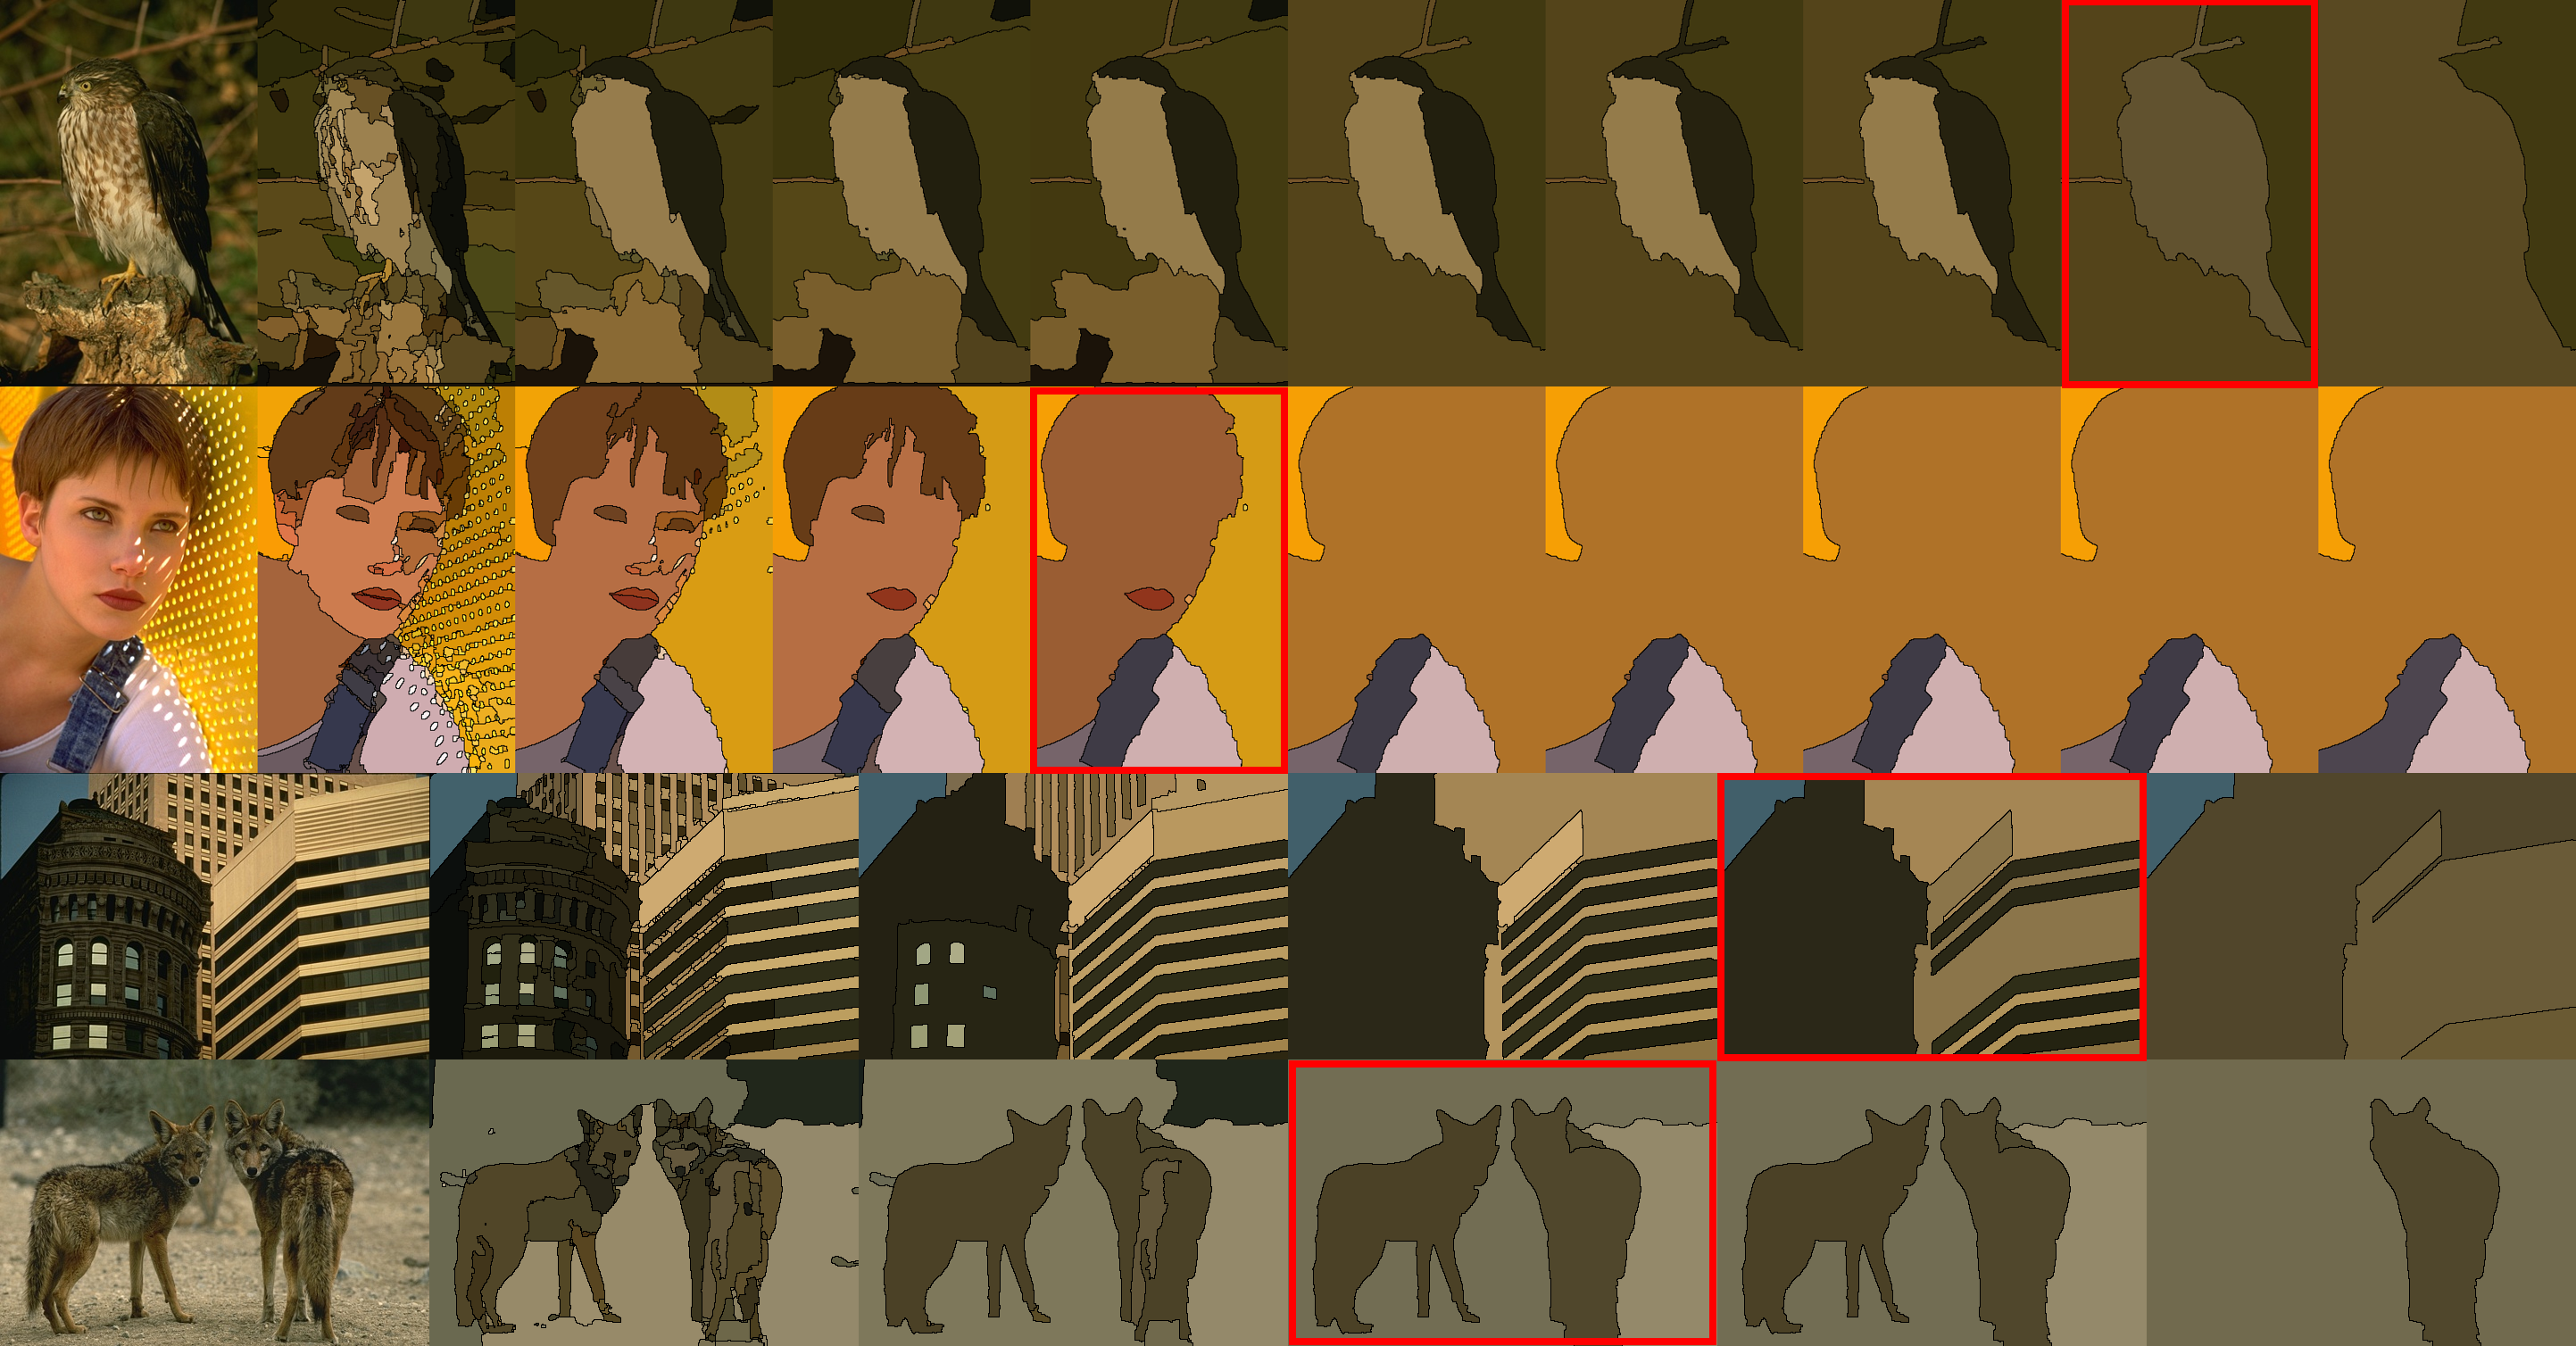
\includegraphics[width=17cm]{fig/vis/stack_1.png} \\
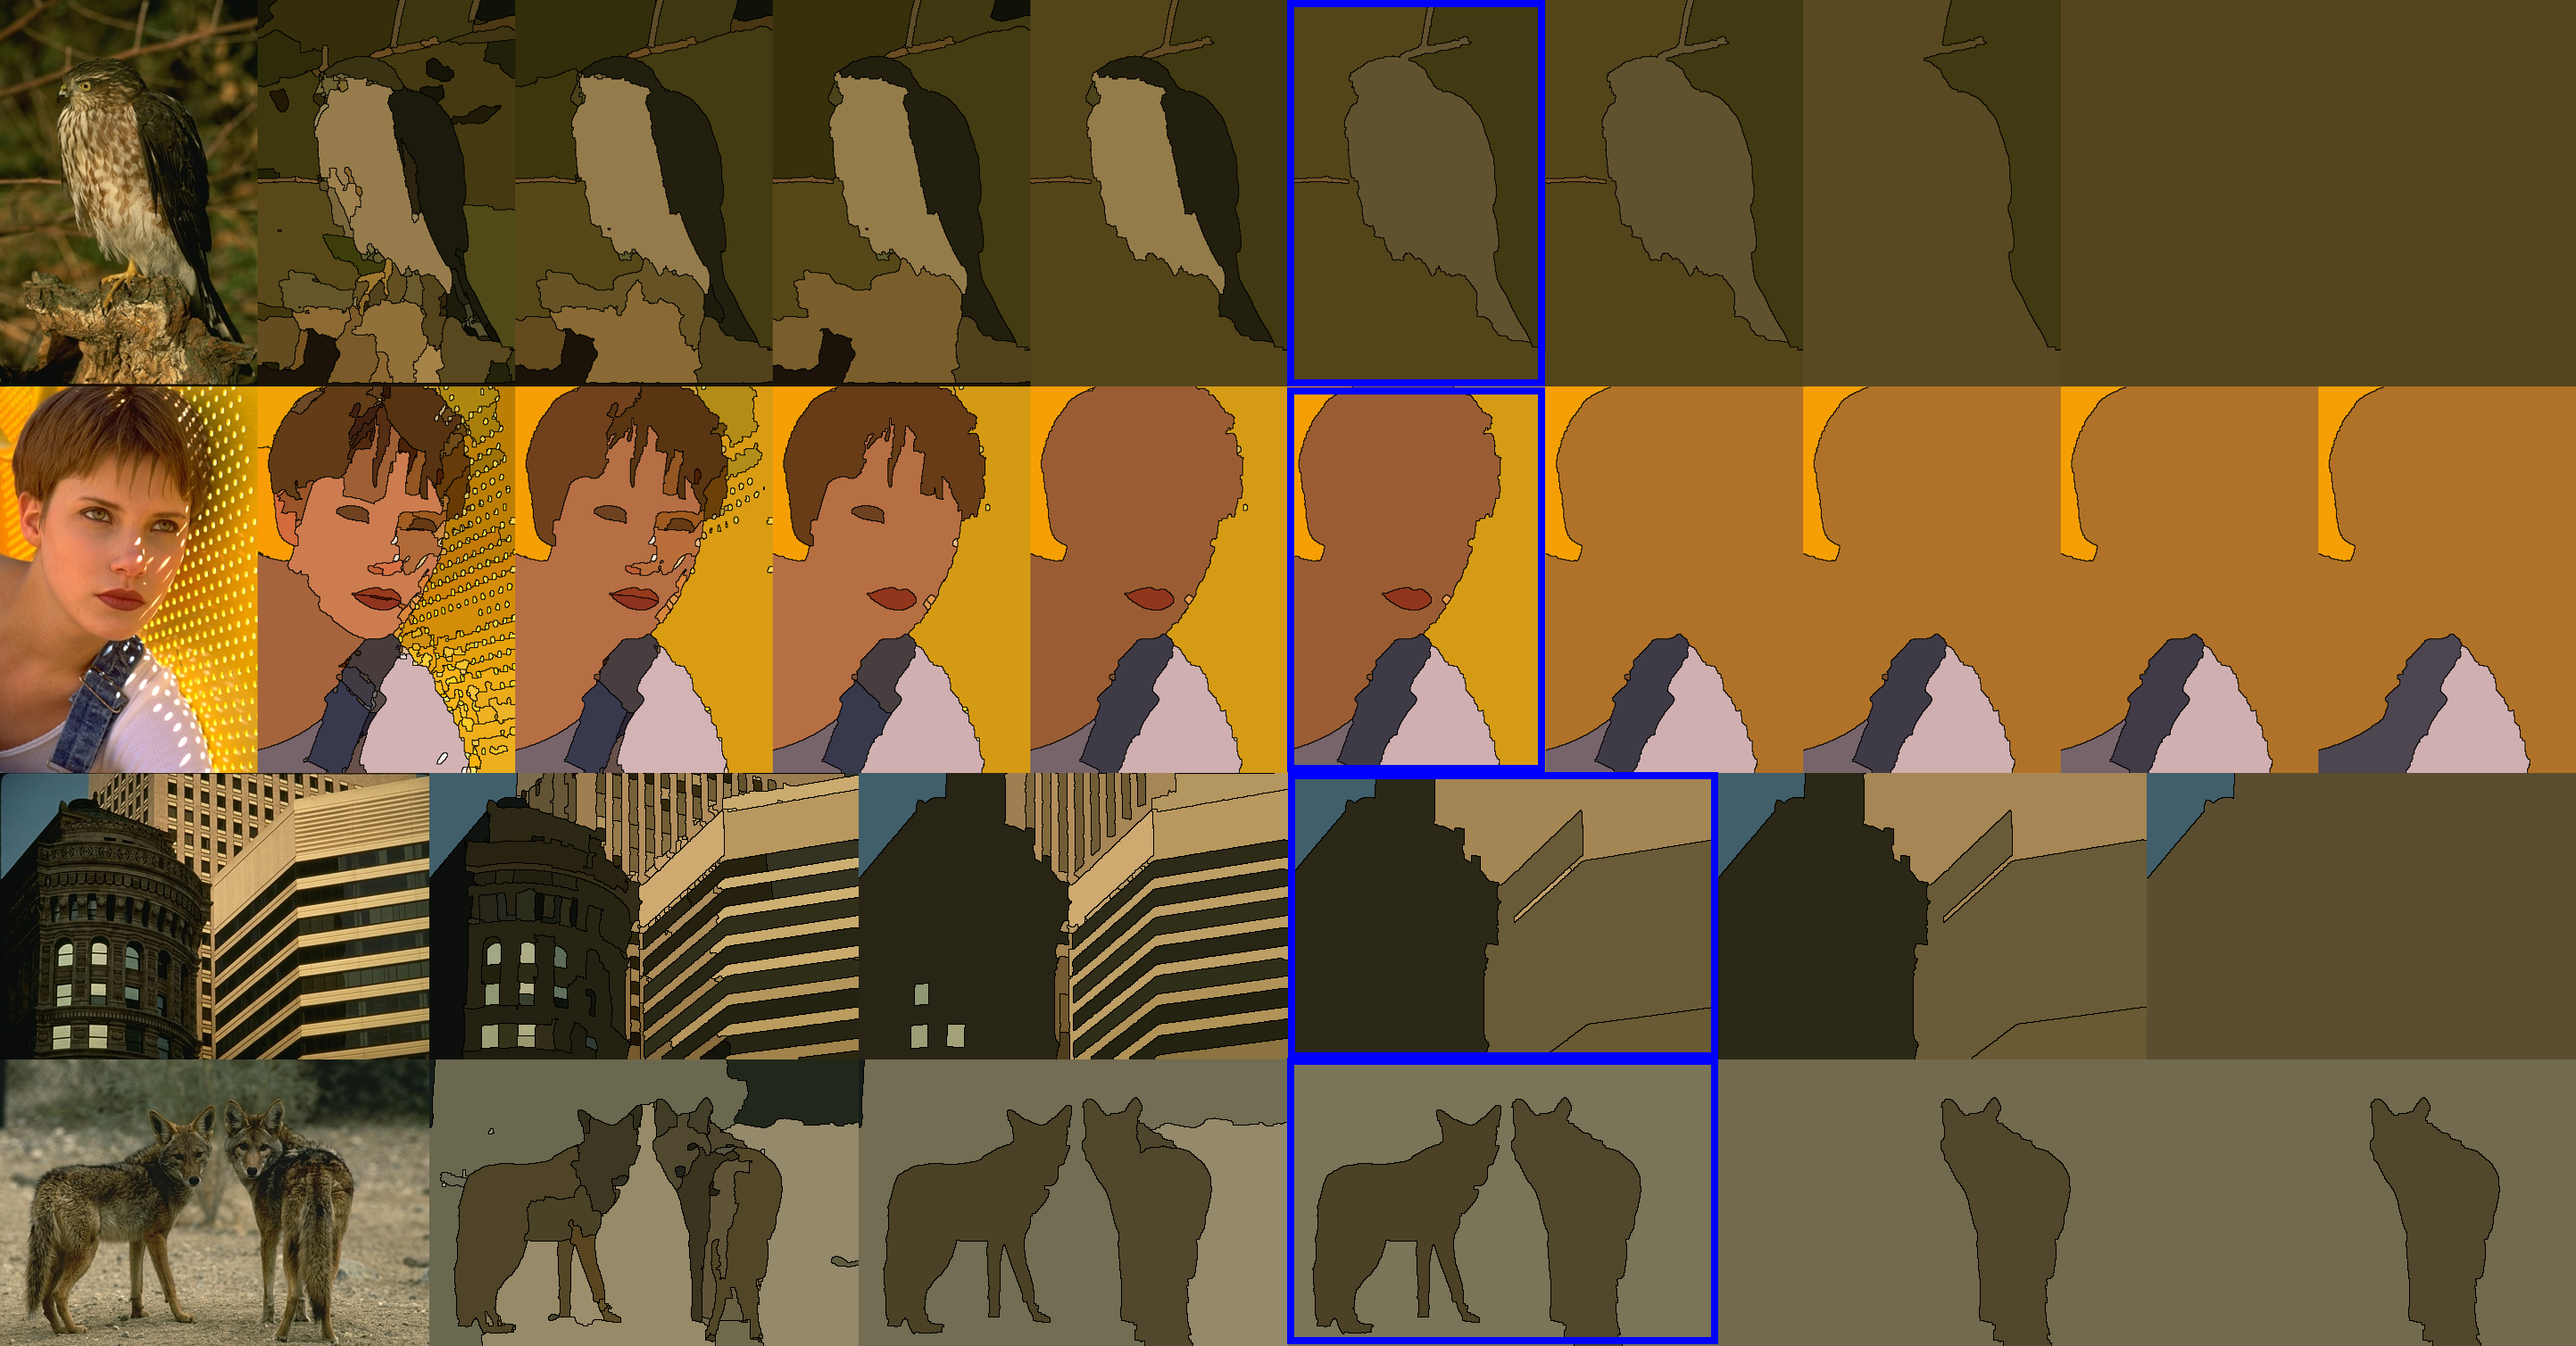
\includegraphics[width=17cm]{fig/vis/stack_2.png}
\end{tabular}
\end{center}
\caption{Results of MCG(first row) and MCG results improved by our approach(second row). Original images are shown in the left most. Segmentations of optimal-dataset-sclae(ODS) are given in the middle. And from left to right are different scales, from fine to coarse. Red bounding box indicates the scale with best results achieved by MCG, and blue box for ours. It can be seen that our approach provides better alignment, both across images and within one image. }
\label{fig:mcg_vis2}
\end{figure*}


\begin{figure*}
\begin{minipage}{0.32\linewidth}
\resizebox{\linewidth}{!}{%
\begin{tikzpicture}[/pgfplots/width=1.5\linewidth, /pgfplots/height=1.2\linewidth]
    \begin{axis}[ymin=0.2,ymax=0.7,xmin=1,xmax=10,enlargelimits=false,
        xlabel=Number of selected regions,
        ylabel=Jaccard index $J$,
        font=\scriptsize, grid=both,
        legend pos= south east,
        grid style=dotted,
        axis equal image=false,
        title=BSDS500,
        title style={yshift=-1.3ex,},
        ytick={0.1,0.2,...,0.7},
        xtick={1,2,...,10},
        minor ytick={0.1,0.125,...,0.7},
        major grid style={white!20!black},
        minor grid style={white!70!black},
        xlabel shift={-2pt},
        ylabel shift={-3pt}]
         \addplot+[black,solid,mark=none, thick] table[x=mR,y=mJ] {data/BSDS500_val_A-MCG_qual_vs_nregs.txt};
         \addlegendentry{MCG+Our}
         \addplot+[black,dashed,mark=none, thick] table[x=mR,y=mJ] {data/BSDS500_val_MCG_qual_vs_nregs.txt};
         \addlegendentry{MCG}
         \addplot+[blue,solid,mark=none, thick] table[x=mR,y=mJ] {data/BSDS500_val_A-SCG_qual_vs_nregs.txt};
         \addlegendentry{SCG+Our}
         \addplot+[blue,dashed,mark=none, thick] table[x=mR,y=mJ] {data/BSDS500_val_SCG_qual_vs_nregs.txt};
         \addlegendentry{SCG}
         \addplot+[red,solid,mark=none, thick] table[x=mR,y=mJ] {data/BSDS500_val_A-gPb-UCM_qual_vs_nregs.txt};
         \addlegendentry{gPb-UCM+Our}
         \addplot+[red,dashed,mark=none, thick] table[x=mR,y=mJ] {data/BSDS500_val_gPb-UCM_qual_vs_nregs.txt};
         \addlegendentry{gPb-UCM}
         \addplot+[olive,solid,mark=none, thick] table[x=mR,y=mJ] {data/BSDS500_val_A-PMI_qual_vs_nregs.txt};
         \addlegendentry{PMI+Our}
         \addplot+[olive,dashed,mark=none, thick] table[x=mR,y=mJ] {data/BSDS500_val_PMI2_qual_vs_nregs.txt};
         \addlegendentry{PMI}
	 \end{axis}
   \end{tikzpicture}}
   \end{minipage}
   \begin{minipage}{0.32\linewidth}
\resizebox{\linewidth}{!}{%
\begin{tikzpicture}[/pgfplots/width=1.5\linewidth, /pgfplots/height=1.2\linewidth]
    \begin{axis}[ymin=0.2,ymax=0.7,xmin=1,xmax=10,enlargelimits=false,
        xlabel=Number of selected regions,
        ylabel=Jaccard index $J$,
        font=\scriptsize, grid=both,
        legend pos= south east,
        grid style=dotted,
        title=Pascal Segmentation,
        title style={yshift=-1.3ex,},
        axis equal image=false,
        ytick={0.1,0.2,...,0.7},
        xtick={1,2,...,10},
        minor ytick={0.1,0.125,...,0.7},
        major grid style={white!20!black},
        minor grid style={white!70!black},
        xlabel shift={-2pt},
        ylabel shift={-3pt}]
         \addplot+[black,solid,mark=none, thick] table[x=mR,y=mJ] {data/Pascal_Segmentation_val_2012_A-MCG3_qual_vs_nregs.txt};
         \addlegendentry{MCG+Our}
         \addplot+[black,dashed,mark=none, thick] table[x=mR,y=mJ] {data/Pascal_Segmentation_val_2012_MCG_qual_vs_nregs.txt};
         \addlegendentry{MCG}
%         \addplot+[red,solid,mark=none, thick] table[x=mR,y=mJ] {data/BSDS500_val_A-gPb-UCM_qual_vs_nregs.txt};
%         \addlegendentry{gPb-UCM+Our}
%         \addplot+[red,dashed,mark=none, thick] table[x=mR,y=mJ] {data/BSDS500_val_gPb-UCM_qual_vs_nregs.txt};
	 \end{axis}
   \end{tikzpicture}}
   \end{minipage}
      \begin{minipage}{0.32\linewidth}
\resizebox{\linewidth}{!}{%
\begin{tikzpicture}[/pgfplots/width=1.5\linewidth, /pgfplots/height=1.2\linewidth]
    \begin{axis}[ymin=0.2,ymax=0.7,xmin=1,xmax=10,enlargelimits=false,
        xlabel=Number of selected regions,
        ylabel=Jaccard index $J$,
        font=\scriptsize, grid=both,
        legend pos= south east,
        grid style=dotted,
        title=MS COCO,
        title style={yshift=-1.3ex,},
        axis equal image=false,
        ytick={0.1,0.2,...,0.7},
        xtick={1,2,...,10},
        minor ytick={0.1,0.125,...,0.7},
        major grid style={white!20!black},
        minor grid style={white!70!black},
        xlabel shift={-2pt},
        ylabel shift={-3pt}]
         \addplot+[black,solid,mark=none, thick] table[x=mR,y=mJ] {data/COCO_val2014_A-MCG_qual_vs_nregs.txt};
         \addlegendentry{MCG+Our}
         \addplot+[black,dashed,mark=none, thick] table[x=mR,y=mJ] {data/COCO_val2014_MCG_qual_vs_nregs.txt};
         \addlegendentry{MCG}
%         \addplot+[red,solid,mark=none, thick] table[x=mR,y=mJ] {data/BSDS500_val_A-gPb-UCM_qual_vs_nregs.txt};
%         \addlegendentry{gPb-UCM+Our}
%         \addplot+[red,dashed,mark=none, thick] table[x=mR,y=mJ] {data/BSDS500_val_gPb-UCM_qual_vs_nregs.txt};
	 \end{axis}
   \end{tikzpicture}}
   \end{minipage}
   \caption{\textbf{Flattened hierarchies for object detection}: Achievable quality by an oracle with respect to the number of regions needed}
   \label{fig:qual_vs_regs}
\end{figure*}


\begin{figure*}[tb]
\begin{center}
\begin{tabular}{ c  c  c  c  c  c  c }
Image & gpb & gpb+ours & SCG & SCG+ours & MCG & MCG + ours \\
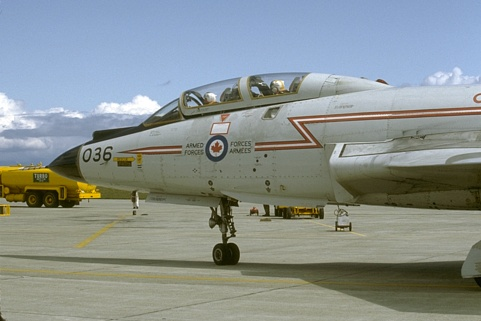
\includegraphics[width=2cm]{fig/visual_result/visual_result_1_1.png}
&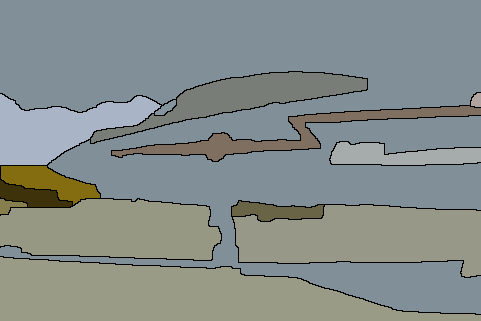
\includegraphics[width=2cm]{fig/visual_result/visual_result_1_2.png}
&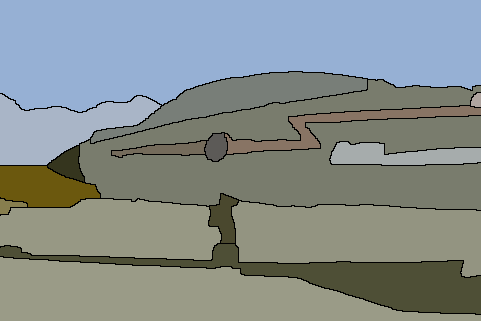
\includegraphics[width=2cm]{fig/visual_result/visual_result_1_3.png}
&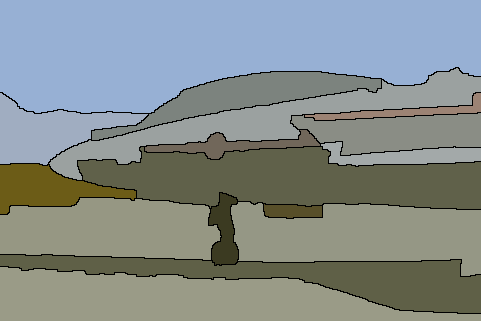
\includegraphics[width=2cm]{fig/visual_result/visual_result_1_4.png}
&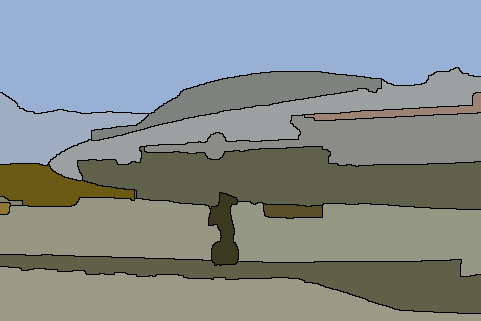
\includegraphics[width=2cm]{fig/visual_result/visual_result_1_5.png}
&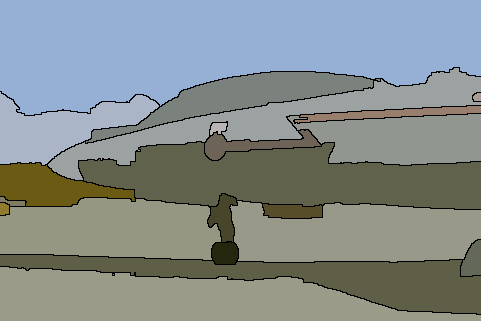
\includegraphics[width=2cm]{fig/visual_result/visual_result_1_6.png}
&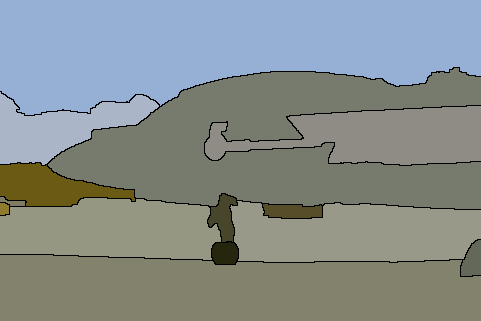
\includegraphics[width=2cm]{fig/visual_result/visual_result_1_7.png}
\\
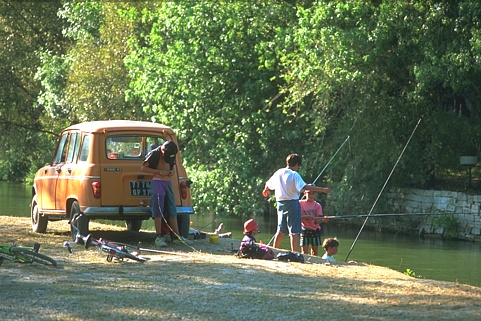
\includegraphics[width=2cm]{fig/visual_result/visual_result_2_1.png}
&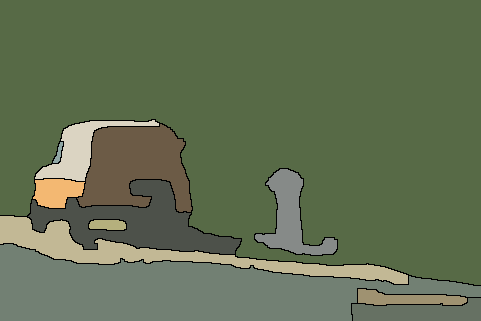
\includegraphics[width=2cm]{fig/visual_result/visual_result_2_2.png}
&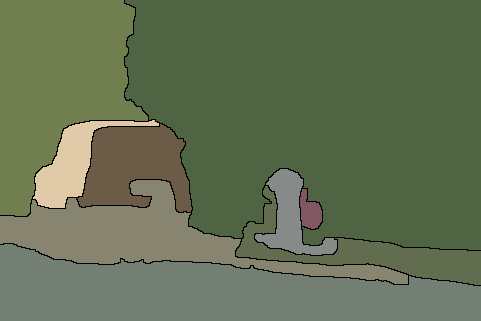
\includegraphics[width=2cm]{fig/visual_result/visual_result_2_3.png}
&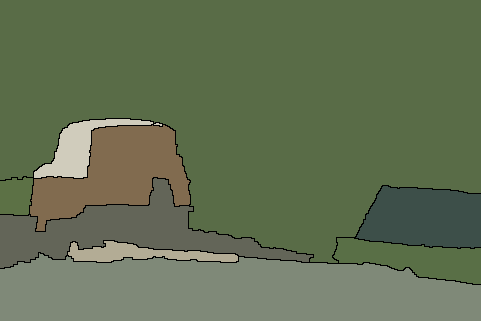
\includegraphics[width=2cm]{fig/visual_result/visual_result_2_4.png}
&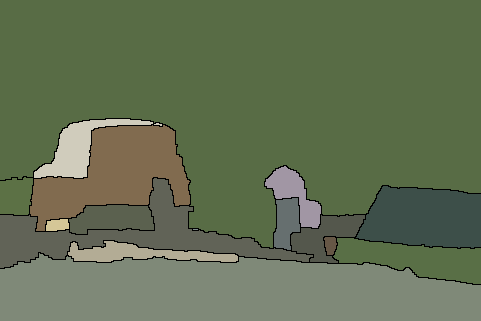
\includegraphics[width=2cm]{fig/visual_result/visual_result_2_5.png}
&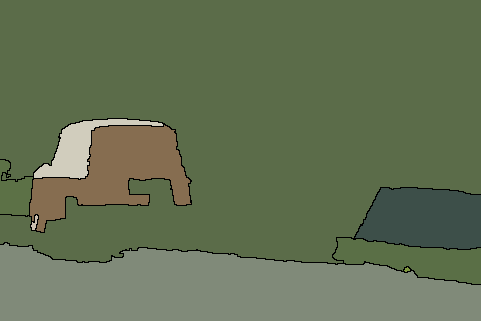
\includegraphics[width=2cm]{fig/visual_result/visual_result_2_6.png}
&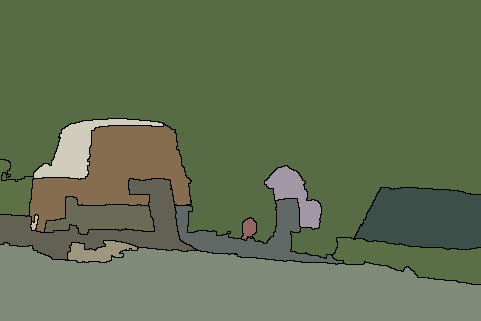
\includegraphics[width=2cm]{fig/visual_result/visual_result_2_7.png}
\\
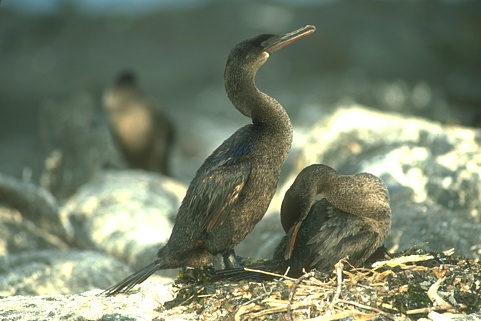
\includegraphics[width=2cm]{fig/visual_result/visual_result_3_1.png}
&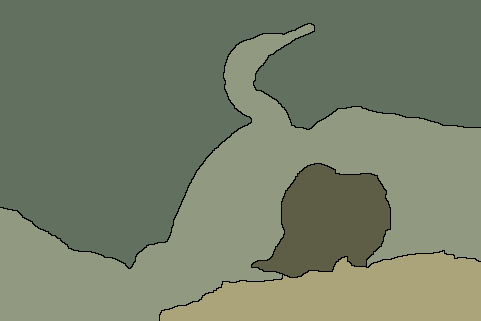
\includegraphics[width=2cm]{fig/visual_result/visual_result_3_2.png}
&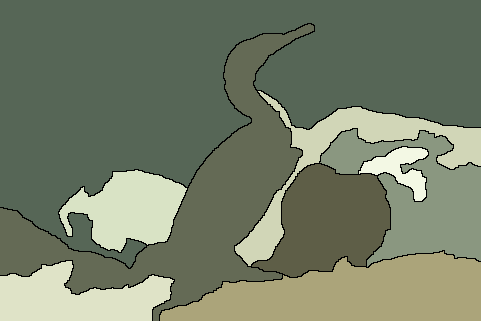
\includegraphics[width=2cm]{fig/visual_result/visual_result_3_3.png}
&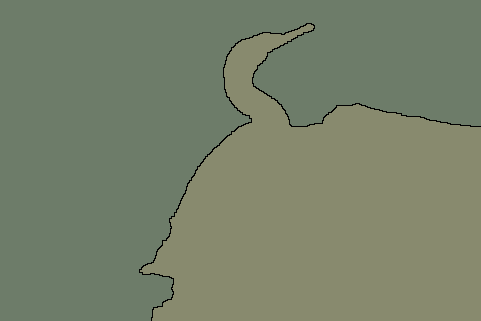
\includegraphics[width=2cm]{fig/visual_result/visual_result_3_4.png}
&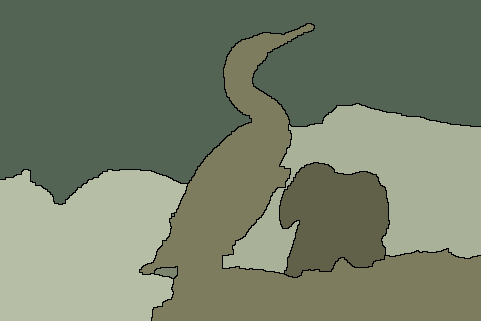
\includegraphics[width=2cm]{fig/visual_result/visual_result_3_5.png}
&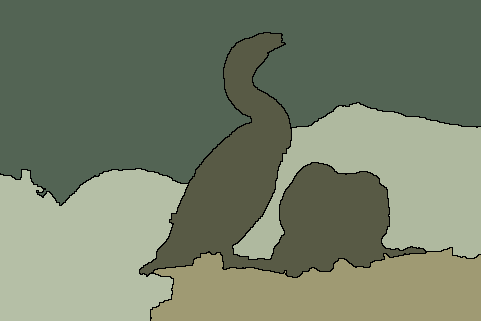
\includegraphics[width=2cm]{fig/visual_result/visual_result_3_6.png}
&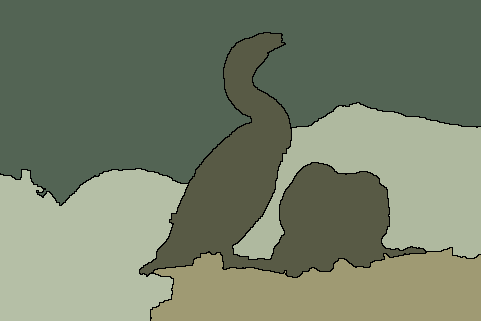
\includegraphics[width=2cm]{fig/visual_result/visual_result_3_7.png}
\\
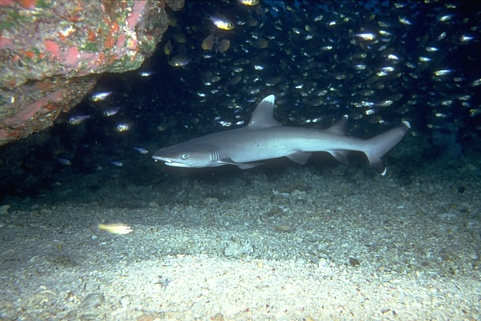
\includegraphics[width=2cm]{fig/visual_result/visual_result_4_1.png}
&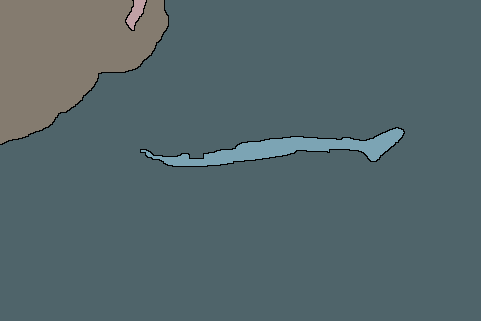
\includegraphics[width=2cm]{fig/visual_result/visual_result_4_2.png}
&
\includegraphics[width=2cm]{fig/visual_result/visual_result_4_3.png}
&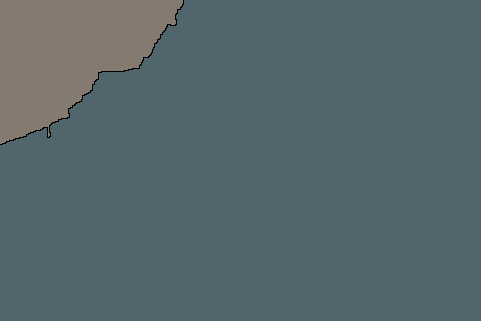
\includegraphics[width=2cm]{fig/visual_result/visual_result_4_4.png}
&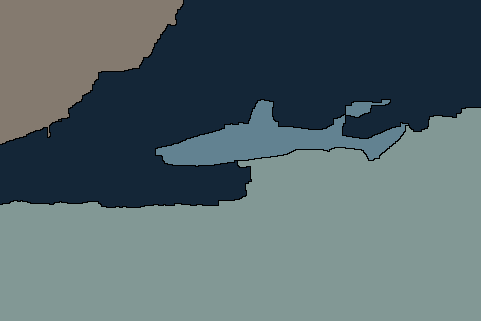
\includegraphics[width=2cm]{fig/visual_result/visual_result_4_5.png}
&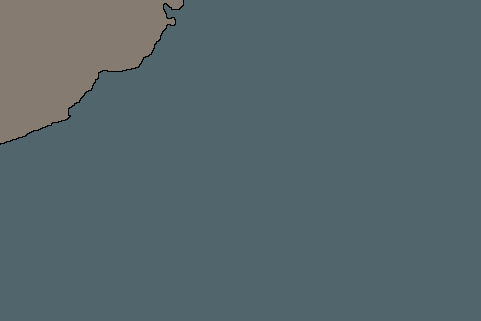
\includegraphics[width=2cm]{fig/visual_result/visual_result_4_6.png}
&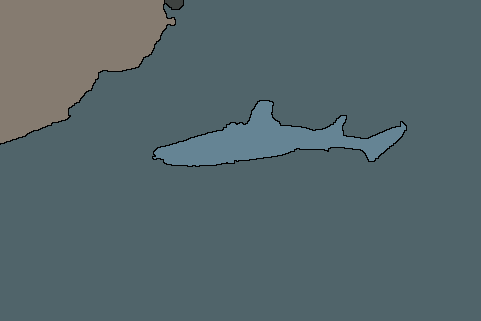
\includegraphics[width=2cm]{fig/visual_result/visual_result_4_7.png}
\\
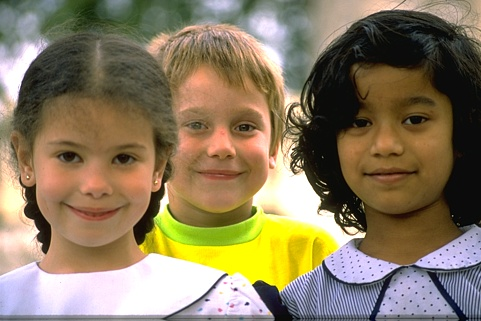
\includegraphics[width=2cm]{fig/visual_result/visual_result_5_1.png}
&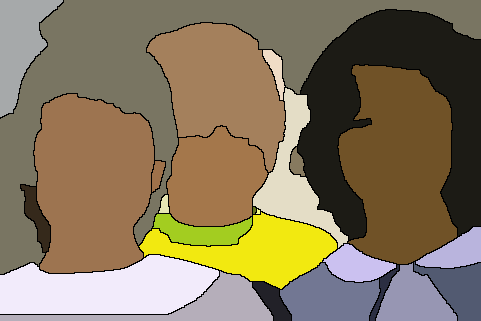
\includegraphics[width=2cm]{fig/visual_result/visual_result_5_2.png}
&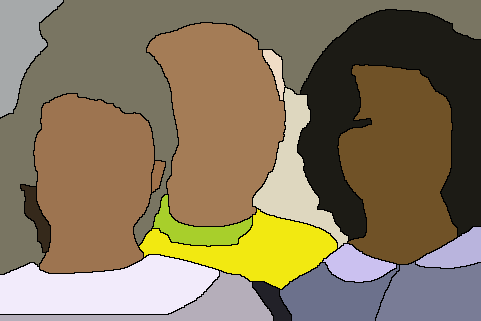
\includegraphics[width=2cm]{fig/visual_result/visual_result_5_3.png}
&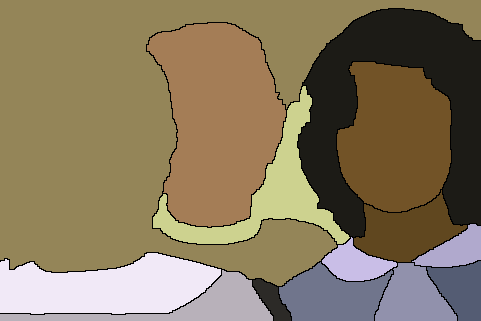
\includegraphics[width=2cm]{fig/visual_result/visual_result_5_4.png}
&\includegraphics[width=2cm]{fig/visual_result/visual_result_5_5.png}
&\includegraphics[width=2cm]{fig/visual_result/visual_result_5_6.png}
&\includegraphics[width=2cm]{fig/visual_result/visual_result_5_7.png}
\\
\includegraphics[width=2cm]{fig/visual_result/visual_result_6_1.png}
&\includegraphics[width=2cm]{fig/visual_result/visual_result_6_2.png}
&\includegraphics[width=2cm]{fig/visual_result/visual_result_6_3.png}
&\includegraphics[width=2cm]{fig/visual_result/visual_result_6_4.png}
&\includegraphics[width=2cm]{fig/visual_result/visual_result_6_5.png}
&\includegraphics[width=2cm]{fig/visual_result/visual_result_6_6.png}
&\includegraphics[width=2cm]{fig/visual_result/visual_result_6_7.png}
\\
\end{tabular}
\end{center}
\caption{Comparison of segmentation results, hierarchies are flattened by optimal dataset scale(ODS).}
\label{fig:visual_result}
\end{figure*}


\subsection{Evaluation towards Object Segmentation}
Segmentation \textit{per se} is rarely the final objective of real
applications, it is rather a middle tool towards, for instance, object
segmentation~\cite{arbelaez2014multiscale} or semantic
segmentation~\cite{Lempitsky2011}.  This section is devoted to show
that better aligned hierarchies also help in this scenario.

In this case we firstly perform the evaluation using the object annotations
provided on the BSDS300 set by~\cite{Endres2014} (we retrain on only BSDS300 train instead of BSDS500).
The intuitive idea is to measure how well we can segment these objects by
\textit{selecting} regions from the different flattened hierarchies.

Figure~\ref{fig:qual_vs_regs} shows the achievable quality
that an oracle could reached if selecting the regions from the
original hierarchies or the ones with our newly-proposed alignment.
The X axis corresponds to the number of needed regions, \ie, the lower
the better.

We can observe that the aligned hierarchies consistently need less
regions to get the same quality in all the tested hierarchies.  In
PMI, for instance, we need to select 5 regions to achieve the same
quality that we can get with 4 on the aligned hierarchy. The
combinatorial space of all possible 4-region combinations is
significantly smaller and thus the search is more probable to
succeed. On the other direction, if we limit the number of regions we
get improvements up to 3 points (9\%) in the achievable quality.

To further illustrates the scalability of the hierarchy alignment on larger dataset, we evaluated our alignment algorithm on Pascal VOC 2012 Segmentation set~\cite{everingham2010pascal} and Microsoft COCO~\cite{lin2014microsoft}. We retrain our scale predictor using the training set of Pascal 2012. In Pascal 2012 dataset, only the segmentation of foreground objects are given, in contrast to BSDS which is fully annotated. Thus during training we only consider all the segments that have overlap with foreground object annotations. The scale predictor is trained as described in Sec~\ref{sec:scale}, the only difference is that $\mathbf{g}$ can only be foreground object. This strategy introduces extra bias towards foreground objects, because no information about the scale of background is given in the training process. However, we are still able to improve alignment of segmentation hierarchies . As shown in Fig\yh{add the figure}, we see that for the range of 2-3 regions (the one in which the MCG object proposal work), the aligned hierarchy provides a 2.5-point improvement ($\sim$6\%), which shows that our method generalizes to larger datasets. \yh{describe some coco results}

\subsection{Running Time}
Our approach takes approximately 3 seconds in total for each image, of which $2.39$
seconds are spent on feature extraction from the segments. The prediction
of regression forest takes about $0.45$ seconds, and the dynamic
programming takes $0.05$ seconds for the inference. Finally, $0.11$
seconds are spent for re-scaling the UCM.
All times are measured on a standard desktop machine.


% \begin{figure*}
% \begin{center}
% \begin{tabular}{c}
% \includegraphics[width=17cm]{fig/vis/70090.png} \\
% \includegraphics[width=17cm]{fig/vis/388006.png} \\
% \includegraphics[width=17cm]{fig/vis/48017.png} \\
% \includegraphics[width=17cm]{fig/vis/196062.png}
% \end{tabular}
% \end{center}
% \caption{Results of MCG(first row) and MCG results improved by our approach(second row). Original images are shown in the left most. Segmentations of optimal-dataset-sclae(ODS) are given in the middle. And from left to right are different scales, from fine to coarse. Red bounding box indicates the scale with best results. It can be seen that our approach provides better alignment, both across images and within one image. }
% \label{fig:mcg_vis1}
% \end{figure*}



\chapter{conclusion} 
\label{ch:conclusion}

wawawa 

{\small
\bibliographystyle{ieee}
\bibliography{egbib}
}

\end{document}
